% Options for packages loaded elsewhere
\PassOptionsToPackage{unicode}{hyperref}
\PassOptionsToPackage{hyphens}{url}
\PassOptionsToPackage{dvipsnames,svgnames,x11names}{xcolor}
%
\documentclass[
  letterpaper,
  DIV=11,
  numbers=noendperiod]{scrartcl}

\usepackage{amsmath,amssymb}
\usepackage{iftex}
\ifPDFTeX
  \usepackage[T1]{fontenc}
  \usepackage[utf8]{inputenc}
  \usepackage{textcomp} % provide euro and other symbols
\else % if luatex or xetex
  \usepackage{unicode-math}
  \defaultfontfeatures{Scale=MatchLowercase}
  \defaultfontfeatures[\rmfamily]{Ligatures=TeX,Scale=1}
\fi
\usepackage{lmodern}
\ifPDFTeX\else  
    % xetex/luatex font selection
\fi
% Use upquote if available, for straight quotes in verbatim environments
\IfFileExists{upquote.sty}{\usepackage{upquote}}{}
\IfFileExists{microtype.sty}{% use microtype if available
  \usepackage[]{microtype}
  \UseMicrotypeSet[protrusion]{basicmath} % disable protrusion for tt fonts
}{}
\makeatletter
\@ifundefined{KOMAClassName}{% if non-KOMA class
  \IfFileExists{parskip.sty}{%
    \usepackage{parskip}
  }{% else
    \setlength{\parindent}{0pt}
    \setlength{\parskip}{6pt plus 2pt minus 1pt}}
}{% if KOMA class
  \KOMAoptions{parskip=half}}
\makeatother
\usepackage{xcolor}
\setlength{\emergencystretch}{3em} % prevent overfull lines
\setcounter{secnumdepth}{-\maxdimen} % remove section numbering
% Make \paragraph and \subparagraph free-standing
\makeatletter
\ifx\paragraph\undefined\else
  \let\oldparagraph\paragraph
  \renewcommand{\paragraph}{
    \@ifstar
      \xxxParagraphStar
      \xxxParagraphNoStar
  }
  \newcommand{\xxxParagraphStar}[1]{\oldparagraph*{#1}\mbox{}}
  \newcommand{\xxxParagraphNoStar}[1]{\oldparagraph{#1}\mbox{}}
\fi
\ifx\subparagraph\undefined\else
  \let\oldsubparagraph\subparagraph
  \renewcommand{\subparagraph}{
    \@ifstar
      \xxxSubParagraphStar
      \xxxSubParagraphNoStar
  }
  \newcommand{\xxxSubParagraphStar}[1]{\oldsubparagraph*{#1}\mbox{}}
  \newcommand{\xxxSubParagraphNoStar}[1]{\oldsubparagraph{#1}\mbox{}}
\fi
\makeatother


\providecommand{\tightlist}{%
  \setlength{\itemsep}{0pt}\setlength{\parskip}{0pt}}\usepackage{longtable,booktabs,array}
\usepackage{calc} % for calculating minipage widths
% Correct order of tables after \paragraph or \subparagraph
\usepackage{etoolbox}
\makeatletter
\patchcmd\longtable{\par}{\if@noskipsec\mbox{}\fi\par}{}{}
\makeatother
% Allow footnotes in longtable head/foot
\IfFileExists{footnotehyper.sty}{\usepackage{footnotehyper}}{\usepackage{footnote}}
\makesavenoteenv{longtable}
\usepackage{graphicx}
\makeatletter
\newsavebox\pandoc@box
\newcommand*\pandocbounded[1]{% scales image to fit in text height/width
  \sbox\pandoc@box{#1}%
  \Gscale@div\@tempa{\textheight}{\dimexpr\ht\pandoc@box+\dp\pandoc@box\relax}%
  \Gscale@div\@tempb{\linewidth}{\wd\pandoc@box}%
  \ifdim\@tempb\p@<\@tempa\p@\let\@tempa\@tempb\fi% select the smaller of both
  \ifdim\@tempa\p@<\p@\scalebox{\@tempa}{\usebox\pandoc@box}%
  \else\usebox{\pandoc@box}%
  \fi%
}
% Set default figure placement to htbp
\def\fps@figure{htbp}
\makeatother

\KOMAoption{captions}{tableheading}
\makeatletter
\@ifpackageloaded{caption}{}{\usepackage{caption}}
\AtBeginDocument{%
\ifdefined\contentsname
  \renewcommand*\contentsname{Table of contents}
\else
  \newcommand\contentsname{Table of contents}
\fi
\ifdefined\listfigurename
  \renewcommand*\listfigurename{List of Figures}
\else
  \newcommand\listfigurename{List of Figures}
\fi
\ifdefined\listtablename
  \renewcommand*\listtablename{List of Tables}
\else
  \newcommand\listtablename{List of Tables}
\fi
\ifdefined\figurename
  \renewcommand*\figurename{Figure}
\else
  \newcommand\figurename{Figure}
\fi
\ifdefined\tablename
  \renewcommand*\tablename{Table}
\else
  \newcommand\tablename{Table}
\fi
}
\@ifpackageloaded{float}{}{\usepackage{float}}
\floatstyle{ruled}
\@ifundefined{c@chapter}{\newfloat{codelisting}{h}{lop}}{\newfloat{codelisting}{h}{lop}[chapter]}
\floatname{codelisting}{Listing}
\newcommand*\listoflistings{\listof{codelisting}{List of Listings}}
\makeatother
\makeatletter
\makeatother
\makeatletter
\@ifpackageloaded{caption}{}{\usepackage{caption}}
\@ifpackageloaded{subcaption}{}{\usepackage{subcaption}}
\makeatother

\usepackage{bookmark}

\IfFileExists{xurl.sty}{\usepackage{xurl}}{} % add URL line breaks if available
\urlstyle{same} % disable monospaced font for URLs
\hypersetup{
  pdftitle={STA304 Report},
  pdfauthor={Chau Nguyen, John Luc, Adam Tadj, Sunwoo Hwang, Sabrina Seiler},
  colorlinks=true,
  linkcolor={blue},
  filecolor={Maroon},
  citecolor={Blue},
  urlcolor={Blue},
  pdfcreator={LaTeX via pandoc}}


\title{STA304 Report}
\author{Chau Nguyen, John Luc, Adam Tadj, Sunwoo Hwang, Sabrina Seiler}
\date{2024-12-02}

\begin{document}
\maketitle


\section{1. Abstract}\label{abstract}

University students frequently face challenges that contribute to mental
health issues such as stress and anxiety. This study examines the
relationship between mental health and factors such as academic
workload, hours of sleep, living situation, and work-life balance. Data
were collected through a Google Form survey administered to students in
a third-year statistics survey \& sampling course, where participants
rated their agreement with statements related to various mental health
indicators. The results showed a significant relationship between
academic workload and stress levels. While no significant relationship
was found between stress levels and hours of sleep, we observed a
significant association between hours of sleep and missed social events.
Additionally, no statistically significant relationship was identified
between stress levels and living situation, though a marginally
significant relationship was found between living situation and missed
social events. Since we were not able to reach most of the conclusions
that we expected, we plan to consider other factors that might influence
mental health, and also incorporate attention-check questions to
identify rushed responses.

\section{2. Introduction}\label{introduction}

The academic workload faced by university students has increasingly
become one of the critical variables for university students concerning
mental health. Given a broader context of increasing academic
challenges, many students experience heightened stress levels, which
impact various aspects of their well-being, including sleep quality,
work-life balance, and several mental health issues.

First, commonly reported mental health issues, including anxiety,
depression and stress, have been found to correlate with academic
pressures in highly competitive or rigorous programs where students may
feel unable to meet academic and personal expectations (Beiter et al.,
2014). Second, research indicates that students experiencing high
academic workload tend to report poorer sleep quality and shorter sleep
duration, which, in turn, can exacerbate mental health problems and
academic performance challenges (Hershner \& Chervin, 2014). Third,
students' living environments and their ability to maintain a balanced
lifestyle can also significantly impact mental health, since living in a
more supportive and conducive environment positions students to better
manage academic responsibilities and personal well-being (Hysing et al.,
2016).

Given the above potential factors, we seek to address the following
research questions in this report:

\begin{itemize}
\item
  \textbf{Research Question 1:} Is there an association between
  students' academic workload and the amount of mental health issues?

  \begin{itemize}
  \item
    \textbf{Null Hypothesis:} There is no association between academic
    workload and the amount of mental health issues.
  \item
    \textbf{Alternative Hypothesis:} There is a significant association
    between academic workload and the amount of mental health issues.
  \end{itemize}
\item
  \textbf{Research Question 2:} How does the academic workload affect
  the quality/length of sleep and its subsequent impact on students'
  mental health?

  \begin{itemize}
  \item
    \textbf{Null Hypothesis:} Academic workload does not affect the
    quality or length of sleep, nor does it affect students' mental
    health.
  \item
    \textbf{Alternative Hypothesis:} Academic workload significantly
    affects the quality and/or amount of sleep students get, which
    affects mental health.
  \end{itemize}
\item
  \textbf{Research Question 3:} Is mental health affected by students'
  living situations or students' ability to maintain work-life balance?

  \begin{itemize}
  \item
    \textbf{Null Hypothesis:} Students' mental health is not affected by
    their living situation or their ability to maintain a work-life
    balance.
  \item
    \textbf{Alternative Hypothesis:} Students' mental health is
    significantly affected by their living situation and their ability
    to maintain a work-life balance.
  \end{itemize}
\end{itemize}

This study focuses on students enrolled in STA304H5 during Fall 2024,
aiming to provide valuable insights into the effects of academic
workload on their overall well-being. By exploring these relationships,
the findings may inform strategies to enhance student support services
and improve academic experiences.

\section{3. Methodology}\label{methodology}

\subsection{3.1. Data Collection}\label{data-collection}

Between October 8th, 2024, and October 20th, 2024, the questionnaire's
Google Form link was posted on the STA304H5 Piazza course discussion
board. We utilized Simple Random Sampling (SRS) by using the R random
generator to randomly sample 45 students from the received questionnaire
responses. This method was chosen because it gives all respondents an
equal chance of being included in the sample, making the sample
representative. This experiment does not require methods like stratified
or cluster sampling because the population in this experiment is
relatively uniform and doesn't need to be divided into strata or
clusters.

We considered alternative methods, such as stratified sampling or
cluster sampling. However, these methods are more suitable when the
characteristics of specific subpopulations need to be accounted for.
Since the characteristics of students taking STA304 were expected to be
similar, we decided that it would not be meaningful to distinguish
between the subpopulations. Since our goal was to capture the
characteristics of all students, we determined that SRS was the most
appropriate method for this experiment.

On the questionnaire, we asked participants to complete 10 short-answer
questions inquiring about academic workload, average hours studied
weekly, amounts of experienced stress-related symptoms (stress, anxiety,
concentration difficulty), hours of sleep per night, current living
situation, and experienced common issues caused by academic workload
(time management, social life, financial).

\subsection{3.2. Target Population}\label{target-population}

The target population consists of students enrolled in the STA304H5
course during the Fall 2024 semester.

\subsection{3.3. Sampling Method}\label{sampling-method}

We will use \textbf{Simple Random Sampling (SRS)} by combining both
sections of the STA304H5 course and selecting a random sample of
students from the pool.

\subsection{3.4. Variables of interest}\label{variables-of-interest}

The following variables were identified for the research:

\subsubsection{3.4.1. Academic Workload}\label{academic-workload}

Academic workload is defined as the number of assignments, projects, and
exams and the overall demands of a course. The purpose of this study is
to see if a high academic workload is associated with increased mental
health problems, such as stress. Academic workload was measured through
a questionnaire on a scale of 1 (very light), 2 (light), 3 (moderate), 4
(heavy) and 5 (very heavy).

\subsubsection{3.4.2. Living Situation}\label{living-situation}

We divided students' living arrangements into four categories: Living
alone, living with family, living with roommates, and living in
on-campus housing. These living arrangements are important variables
that have a significant impact on students' mental health and academic
stress.

\subsubsection{3.4.3. Study Hours}\label{study-hours}

Study time is an important indicator of students' time management and
academic performance. This study analyzes the relationship between study
time and mental health , exploring whether over studying leads to stress
reduction or instead causes mental stress and anxiety. Study hours were
measured by entering the number of hours of study per week.

\subsubsection{3.4.4. Mental Health Symptoms (Stress, Anxiety, and
Concentration
Difficulties)}\label{mental-health-symptoms-stress-anxiety-and-concentration-difficulties}

Mental health symptoms are key indicators of students' mental health and
may be influenced by academic workload and living conditions.
Understanding these relationships helps target interventions and support
strategies to improve students' mental well-being. These symptoms were
measured through a questionnaire on a scale of 1 (Never) 2 (Sometimes)
and 3 (Always).

\subsubsection{3.4.5. Work-life balance Factors (Financials, Time
Management)}\label{work-life-balance-factors-financials-time-management}

Two key indicators of how well a student is adjusting to an independent
life in university is their financial status and ability to manage time
properly. Therefore, we believe that investing these factors would help
to shed light on whether students' work-life balance are being impacted
by academic workload. These are measured through a questionnaire of how
often students feel these factors are of concern as a result of their
workload, on a scale of 1-5 (Never, Rarely, Sometimes, Often, Very
Often).

\subsection{3.5. Sample Size}\label{sample-size}

In our research, we applied Simple Random Sampling (SRS) on 200
students. To determine the sample size using the bound of error as 0.29,
we used the following formula to find the magnitude of the confidence
interval: \[
D = \frac{B^2}{4}
\]

Where \(B = 0.29\), giving: \[
D = \frac{(0.29)^2}{4} = 0.021025
\]

Using the standard deviation (\(\sigma\)) of the academic workload
variable, we computed the required sample size using the formula: \[
n = \frac{N \times \sigma^2}{(N-1) \times D + \sigma^2}
\] Where:

N = 200 (total population size) B = 0.29 (bound of error) D = B²/4 =
0.021025 \(\sigma\) is approximated as (range of academic workload)/4
range = maximum academic workload - minimum academic workload

To randomize our sampling process, we used R's random sampling function
\(\texttt{sample()}\) with a fixed \(\texttt{seed}\)
(\(\texttt{set.seed(1)}\)) to randomly select participants from the full
dataset based on the calculated sample size n.

Thus, below is the initial setup for all of our statistical tests.

\section{4. Analysis}\label{analysis}

\subsection{4.1. Analysis of Variance
(ANOVA)}\label{analysis-of-variance-anova}

RQ1 questions if academic workload contributes to a student's stress
levels. To answer this question, ANOVA (analysis of variance) is used to
test the difference in average stress levels between students with
different academic workloads.

All our assumptions are satisfied, as (1) samples between the groups
were randomly sampled and responses are independent from each other, (2)
data from each group is normally distributed (large sample size, \(n\)
\textgreater{} 30), and (3) variances are approximately equal (obtained
\emph{p-value} of 0.07758 from Barlett's test, which is above the
significance level \(\alpha = 0.05\).) All categories were converted to
categorical data to make them suitable for ANOVA testing.

\subsubsection{4.1.1. ANOVA between stress and academic
workload}\label{anova-between-stress-and-academic-workload}

\begin{longtable}[]{@{}
  >{\raggedright\arraybackslash}p{(\linewidth - 10\tabcolsep) * \real{0.1892}}
  >{\raggedright\arraybackslash}p{(\linewidth - 10\tabcolsep) * \real{0.2252}}
  >{\raggedright\arraybackslash}p{(\linewidth - 10\tabcolsep) * \real{0.1982}}
  >{\raggedright\arraybackslash}p{(\linewidth - 10\tabcolsep) * \real{0.1622}}
  >{\raggedright\arraybackslash}p{(\linewidth - 10\tabcolsep) * \real{0.0811}}
  >{\raggedright\arraybackslash}p{(\linewidth - 10\tabcolsep) * \real{0.1441}}@{}}
\toprule\noalign{}
\begin{minipage}[b]{\linewidth}\raggedright
Variable
\end{minipage} & \begin{minipage}[b]{\linewidth}\raggedright
Degrees of Freedom (DF)
\end{minipage} & \begin{minipage}[b]{\linewidth}\raggedright
Sum of Squares (SS)
\end{minipage} & \begin{minipage}[b]{\linewidth}\raggedright
Mean Square (MS)
\end{minipage} & \begin{minipage}[b]{\linewidth}\raggedright
F-value
\end{minipage} & \begin{minipage}[b]{\linewidth}\raggedright
Pr(\textgreater F)
\end{minipage} \\
\midrule\noalign{}
\endhead
\bottomrule\noalign{}
\endlastfoot
academic workload & 3 & 3.136 & 1.0455 & 4.273 & 0.0136 \\
Residuals & 27 & 6.605 & 0.2446 & & \\
\end{longtable}

For the relationship between stress and academic workload, we divided
the criteria of stress into categories of Never, Sometimes, and Always,
and compared each group with an ANOVA test. Since the calculated
\(F-value\) of 5.121 is larger than the critical \(F-value\) of 2.874 at
a 5\% significance level for (3, 35) degrees of freedom, we reject the
null hypothesis. Therefore, there is a statistically significant
relationship between student academic workload and levels of stress.

\subsubsection{4.1.2. ANOVA between stress and hours of
sleep}\label{anova-between-stress-and-hours-of-sleep}

\begin{longtable}[]{@{}
  >{\raggedright\arraybackslash}p{(\linewidth - 10\tabcolsep) * \real{0.1892}}
  >{\raggedright\arraybackslash}p{(\linewidth - 10\tabcolsep) * \real{0.2252}}
  >{\raggedright\arraybackslash}p{(\linewidth - 10\tabcolsep) * \real{0.1982}}
  >{\raggedright\arraybackslash}p{(\linewidth - 10\tabcolsep) * \real{0.1622}}
  >{\raggedright\arraybackslash}p{(\linewidth - 10\tabcolsep) * \real{0.0811}}
  >{\raggedright\arraybackslash}p{(\linewidth - 10\tabcolsep) * \real{0.1441}}@{}}
\toprule\noalign{}
\begin{minipage}[b]{\linewidth}\raggedright
Variable
\end{minipage} & \begin{minipage}[b]{\linewidth}\raggedright
Degrees of Freedom (DF)
\end{minipage} & \begin{minipage}[b]{\linewidth}\raggedright
Sum of Squares (SS)
\end{minipage} & \begin{minipage}[b]{\linewidth}\raggedright
Mean Square (MS)
\end{minipage} & \begin{minipage}[b]{\linewidth}\raggedright
F-value
\end{minipage} & \begin{minipage}[b]{\linewidth}\raggedright
Pr(\textgreater F)
\end{minipage} \\
\midrule\noalign{}
\endhead
\bottomrule\noalign{}
\endlastfoot
sleep & 2 & 1.242 & 0.6210 & 2.046 & 0.148 \\
Residuals & 28 & 8.500 & 0.3036 & & \\
\end{longtable}

In the case of the relationship between Stress and Sleep, we ran an
ANOVA test on sleep hours that have been converted into categorical
data. The hours were divided into 6 hours or less, between 6 and 8
hours, and more than 8 hours. Since the calculated
\[F-value of 0.163 is smaller than the critical $F-value$ of 3.259 at the \]0.05\$
significance level for (2, 36) degrees of freedom, we fail to reject the
null hypothesis.

Therefore, there is no statistically significant relationship between
hours of sleep and levels of stress among students. This suggests that
variations in hours of sleep do not significantly affect variations in
stress levels.

\subsubsection{4.1.3. ANOVA between stress and missed social
events}\label{anova-between-stress-and-missed-social-events}

\begin{longtable}[]{@{}
  >{\raggedright\arraybackslash}p{(\linewidth - 10\tabcolsep) * \real{0.2105}}
  >{\raggedright\arraybackslash}p{(\linewidth - 10\tabcolsep) * \real{0.2193}}
  >{\raggedright\arraybackslash}p{(\linewidth - 10\tabcolsep) * \real{0.1930}}
  >{\raggedright\arraybackslash}p{(\linewidth - 10\tabcolsep) * \real{0.1579}}
  >{\raggedright\arraybackslash}p{(\linewidth - 10\tabcolsep) * \real{0.0789}}
  >{\raggedright\arraybackslash}p{(\linewidth - 10\tabcolsep) * \real{0.1404}}@{}}
\toprule\noalign{}
\begin{minipage}[b]{\linewidth}\raggedright
Variable
\end{minipage} & \begin{minipage}[b]{\linewidth}\raggedright
Degrees of Freedom (DF)
\end{minipage} & \begin{minipage}[b]{\linewidth}\raggedright
Sum of Squares (SS)
\end{minipage} & \begin{minipage}[b]{\linewidth}\raggedright
Mean Square (MS)
\end{minipage} & \begin{minipage}[b]{\linewidth}\raggedright
F-value
\end{minipage} & \begin{minipage}[b]{\linewidth}\raggedright
Pr(\textgreater F)
\end{minipage} \\
\midrule\noalign{}
\endhead
\bottomrule\noalign{}
\endlastfoot
missed\_social\_events & 4 & 1.220 & 0.3049 & 0.93 & 0.462 \\
Residuals & 26 & 8.522 & 0.3278 & & \\
\end{longtable}

To investigate the relationship between stress and missed social events,
we ran an ANOVA test on hours of study that have been converted from
continuous numerical values into categorical data. In particular, we
divided the hours into three ranges: 0-10 hours as ``Low'', 10-20 hours
as ``Medium'' and 20 or more as ``High''.

Since the calculated F-value was 1.092, which is less than the critical
value 2.629 (\emph{df}=4, \emph{df}=34), we fail to reject the null
hypothesis. There isn't enough statistical evidence that there exists an
association between \textbf{stress levels} and \textbf{missed social
events}.

Since the calculated F-value of 1.092 is smaller than the critical
\(F-value\) of 2.649 at the 5\% significance level with (4, 34) degrees
of freedom, we fail to reject the null hypothesis. This conclusion is
also supported by the \emph{p-value} of 0.376, which is greater than the
significance level of 0.05. Therefore, there is no statistically
significant relationship between stress levels and missed social events
among students.

\subsection{4.2. Chi-square Test of
Independence}\label{chi-square-test-of-independence}

Research Question 1 questions if there is a relationship between the
academic workload of a student and their mental health. Research
question 3 questions if there is a relationship between students' living
situation or ability to maintain work-life balance. Our assumption that
the data is randomly sampled holds given our method of sampling outlined
above.

To investigate whether there exists a relationship between these
variables, we use the Chi-squared test of independence with
\(\alpha = 0.05\) as the significance level among a permutation of the
variables of interests (academic workload and mental health symptoms)
and (living situations, work-life balance). In total, 12 Chi-squared
tests were performed, with the results and conclusion as follows:

\textbf{Chi-squared Test between Academic Workload and Stress}
\(\chi^2 = 25.936\), \emph{df} = 6, \emph{p-value} = 0.0002288

Since the calculated \emph{p-value} was 0.0002288 and is less than
\(\alpha = 0.05\), we reject the null hypothesis. There is enough
statistical eviende that there is a significant association between
academic workload and the stress levels of a student.

\textbf{Chi-squared Test between Academic Workload and Anxiety}
\(\chi^2 =14.113\),\emph{df}=6, \emph{p-value} =0.0284

Since the calculated \emph{p-value} was 0.0284 and is less than
\(\alpha = 0.05\), we reject the null hypothesis. There is enough
statistical evidence that there is a significant association between the
academic workload and the anxiety levels of a student.

\textbf{Chi-squared Test between Academic Workload and Concentration}
\(\chi^2 =6.5\), \emph{df}=6, \emph{p-value} =0.3696

Since the calculated \emph{p-value} was 0.3696 and is greater than
\(\alpha = 0.05\), we fail to reject the null hypothesis. There isn't
enough statistical evidence to indicate that the academic workload and
the concentration levels of a student are related.

\textbf{Chi-squared Test between Living Situation and Stress}
\(\chi^2 =4.9936\), \emph{df}=6, \emph{p-value} =0.5446

Since the calculated \emph{p-value} was 0.5446 and is greater than
\(\alpha = 0.05\), we fail to reject the null hypothesis. There isn't
enough statistical evidence that the living situation and the stress
levels of a student are related.

\textbf{Chi-squared Test between Living Situation and Anxiety}
\(\chi^2=6.6042\), \emph{df}=6, \emph{p-value} =0.359

Since the calculated \emph{p-value} was 0.359 and is greater than
\(\alpha=0.05\), we fail to reject the null hypothesis. There isn't
enough statistical evidence that the living situation and the anxiety
levels of a student are related.

\textbf{Chi-squared Test between Living Situation and Concentration}
\(\chi^2\) =2.8773, \emph{df}=6, \emph{p-value} =0.8241

Since the calculated \emph{p-value} was 0.8241 and is greater than
\(\alpha=0.05\), we fail to reject the null hypothesis. There isn't
enough statistical evidence that the living situation and the
concentration levels of a student are related.

\textbf{Chi-squared Test between Time Management and Stress} \(\chi^2\)
=10.894, \emph{df}=8, \emph{p-value} =0.2078

Since the calculated \emph{p-value} was 0.2078 and is greater than
\(\alpha=0.05\), we fail to reject the null hypothesis. There isn't
enough statistical evidence that the time management skills and the
stress levels of a student are related.

\textbf{Chi-squared Test between Time Management and Anxiety} \(\chi^2\)
=6.5567, \emph{df}=8, \emph{p-value} =0.5851

Since the calculated \emph{p-value} was 0.5851 and is greater than
\(\alpha=0.05\), we fail to reject the null hypothesis. There isn't
enough statistical evidence that the time management skills and the
anxiety levels of a student are related.

\textbf{Chi-squared Test between Time Management and Concentration}
\(\chi^2\) =9.3321, \emph{df}=8, \emph{p-value} =0.3151

Since the calculated \emph{p-value} was 0.3151 and is greater than
\(\alpha=0.05\), we fail to reject the null hypothesis. There isn't
enough statistical evidence that the time management skills and the
concentration levels of a student are related.

\textbf{Chi-squared Test between Financials and Stress} \(\chi^2\)
=9.3321, \emph{df}=8, \emph{p-value} =0.7223

Since the calculated \emph{p-value} was 0.3151 and is greater than
\(\alpha=0.05\), we fail to reject the null hypothesis. There isn't
enough statistical evidence that the financial situation and the stress
levels of a student are related.

\textbf{Chi-squared Test between Financials and Anxiety} \(\chi^2\)
=5.3134, \emph{df}=8, \emph{p-value} =0.7236

Since the calculated \emph{p-value} was 0.7236 and is greater than
\(\alpha=0.05\), we fail to reject the null hypothesis. There isn't
enough statistical evidence that the financial situation and the anxiety
levels of a student are related.

\textbf{Chi-squared Test between Financials and Concentration}
\(\chi^2\) =6.1471, \emph{df}=8, \emph{p-value} =0.6308

Since the calculated \emph{p-value} was 0.6308 and is greater than
\(\alpha=0.05\), we fail to reject the null hypothesis. There isn't
enough statistical evidence that the financial situation and the
concentration levels of a student are related.

\subsection{4.3. Simple and Multiple Linear
Regressions}\label{simple-and-multiple-linear-regressions}

This part of the analysis focuses on applying linear regression to
address the three research questions outlined in the introduction. We
will explore whether there is a relationship between students' academic
workload and the prevalence of mental health issues; between academic
workload, the amount of sleep students get, and its impact on mental
health; and finally, between mental health, students' living situations,
and their ability to maintain a work-life balance. All of these
relationships were found to be statistically significant.

\subsection{4.3.1. Research Question 1}\label{research-question-1}

\subsubsection{Relevant Graphs \& Tables}\label{relevant-graphs-tables}

Research Question 1 is concerned with determining whether there is a
relationship between students' academic workload and the prevalence of
mental health issues in students. To answer this question, we start by
plotting a boxplot of academic workload by stress level. This plot
suggests that higher stress levels are associated with a higher academic
workload. On average, students who ``Always'' or ``Sometimes'' feel
stressed tend to have a higher workload than those who ``Never'' feel
stressed.

\begin{center}
\pandocbounded{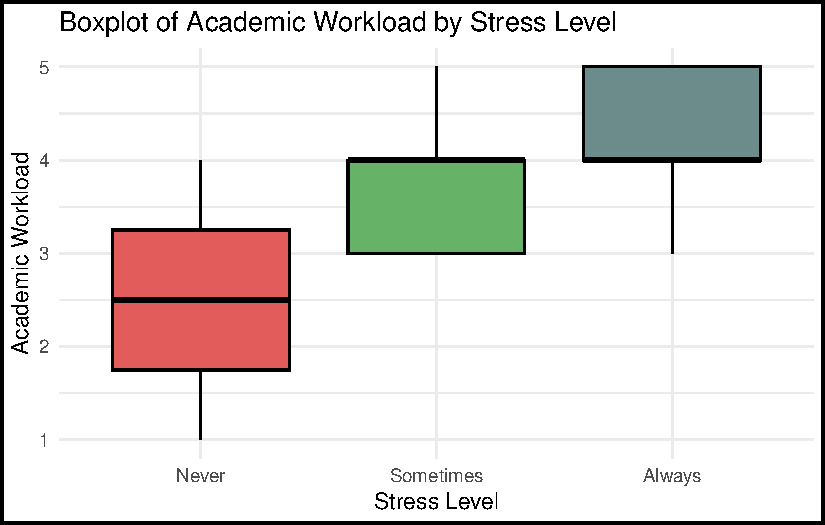
\includegraphics[keepaspectratio]{sta304_report_files/figure-pdf/unnamed-chunk-2-1.pdf}}
\end{center}

\subsubsection{Necessary Assumptions}\label{necessary-assumptions}

To confirm this association, we implement a simple linear regression
model, where the dependent variable is stress\_numeric (the stress
variable, converted to numeric values), and the independent variable is
academic\_workload. To implement this model, we check the following
assumptions using the following plot of the residuals:

\begin{center}
\pandocbounded{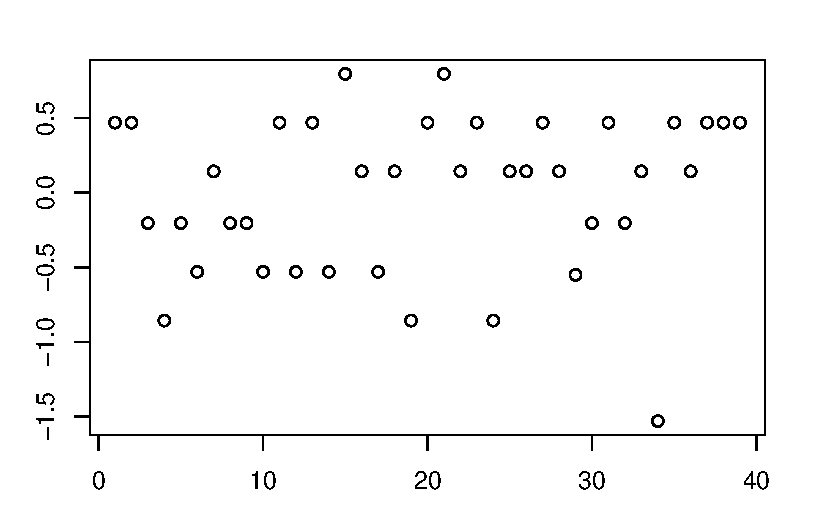
\includegraphics[keepaspectratio]{sta304_report_files/figure-pdf/unnamed-chunk-4-1.pdf}}
\end{center}

\begin{itemize}
\item
  Independence of errors: Since the plot has no noticable pattern, the
  independence assumption is satisfied.
\item
  Normality of errors: Since our sample size is sufficiently large, by
  the Central Limit Theorem the sample mean (and by extension, the
  sampling distribution of residuals) approximately follows a Normal
  distribution.
\item
  Homogeneity of variances amongst errors: Since the residuals plot has
  a ``horizontal band appearance'', this suggests that variance of the
  residuals are the same for all values of the independent variable
  academic\_workload.
\end{itemize}

Since all the assumptions are met, we proceed with the regression
analysis.

\subsubsection{Computation and Statistical Test
Output}\label{computation-and-statistical-test-output}

The regression analysis produced the following results:

\begin{longtable}[]{@{}
  >{\raggedright\arraybackslash}p{(\linewidth - 8\tabcolsep) * \real{0.4118}}
  >{\raggedright\arraybackslash}p{(\linewidth - 8\tabcolsep) * \real{0.1765}}
  >{\raggedright\arraybackslash}p{(\linewidth - 8\tabcolsep) * \real{0.1471}}
  >{\raggedright\arraybackslash}p{(\linewidth - 8\tabcolsep) * \real{0.1324}}
  >{\raggedright\arraybackslash}p{(\linewidth - 8\tabcolsep) * \real{0.1324}}@{}}
\toprule\noalign{}
\begin{minipage}[b]{\linewidth}\raggedright
Statistic
\end{minipage} & \begin{minipage}[b]{\linewidth}\raggedright
Estimate
\end{minipage} & \begin{minipage}[b]{\linewidth}\raggedright
SE
\end{minipage} & \begin{minipage}[b]{\linewidth}\raggedright
t-value
\end{minipage} & \begin{minipage}[b]{\linewidth}\raggedright
\emph{p-value}
\end{minipage} \\
\midrule\noalign{}
\endhead
\bottomrule\noalign{}
\endlastfoot
Intercept (\(\beta_0\)) & 1.22389 & 0.40942 & 2.989 & 0.00495 \\
Slope (\(\beta_1\)) & 0.32655 & 0.09945 & 3.284 & 0.00224 \\
\end{longtable}

\begin{center}\rule{0.5\linewidth}{0.5pt}\end{center}

The residual standard error is \(0.5353\) with \(37\) degrees of
freedom. The \(R^2\) value is \(0.2256\), and the F-statistic is
\(F(1, 37) = 10.78\), with a \emph{p-value} of \(0.002\).

The equation of the regression line is given by: \[
\text{Stress} = 1.22389 + 0.32655 \cdot \text{Academic Workload}
\]

\subsubsection{Interpretation}\label{interpretation}

The small \(p-value = 0.00224\) indicates that academic workload is a
significant predictor of stress. Therefore, we can conclude that there
is a significant relationship between students' academic workload and
their stress levels.

\subsection{4.3.2. Research Question 2}\label{research-question-2}

\subsubsection{Relevant Graphs \&
Tables}\label{relevant-graphs-tables-1}

Research Question 2 investigates whether there is a relationship between
students' academic workload, the amount of sleep they get, and impact on
mental health. Since the ANOVA above showed no significant relationship
between stress and hours of sleep, we investigate the effect of another
factor, the number of missed social events. To begin, we plot a boxplot
of hours of sleep by the number of missed social events. This plot
suggests students who miss more social events tend to have fewer hours
of sleep on average.

\begin{center}
\pandocbounded{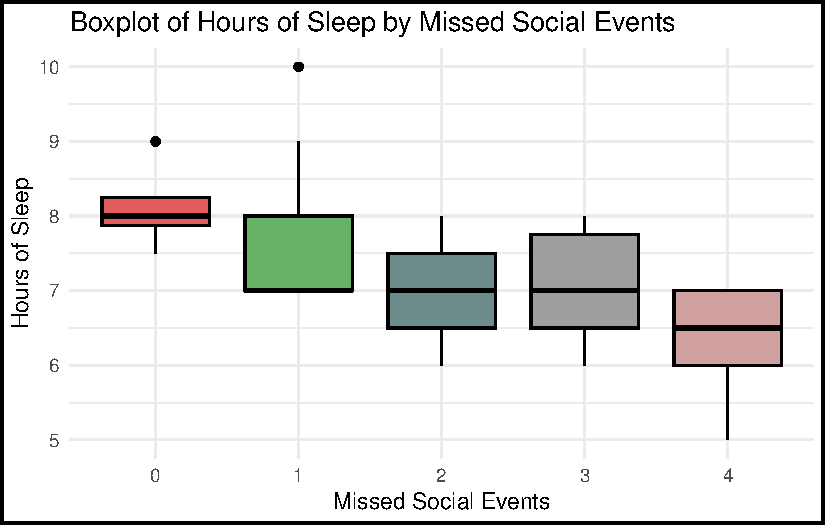
\includegraphics[keepaspectratio]{sta304_report_files/figure-pdf/unnamed-chunk-5-1.pdf}}
\end{center}

\subsubsection{Necessary Assumptions}\label{necessary-assumptions-1}

To assess this relationship, we use a multiple linear regression model
with hours of sleep as the dependent variable, and academic workload and
missed social events as the independent variables. Before interpreting
this model, we check the following assumptions:

\begin{center}
\pandocbounded{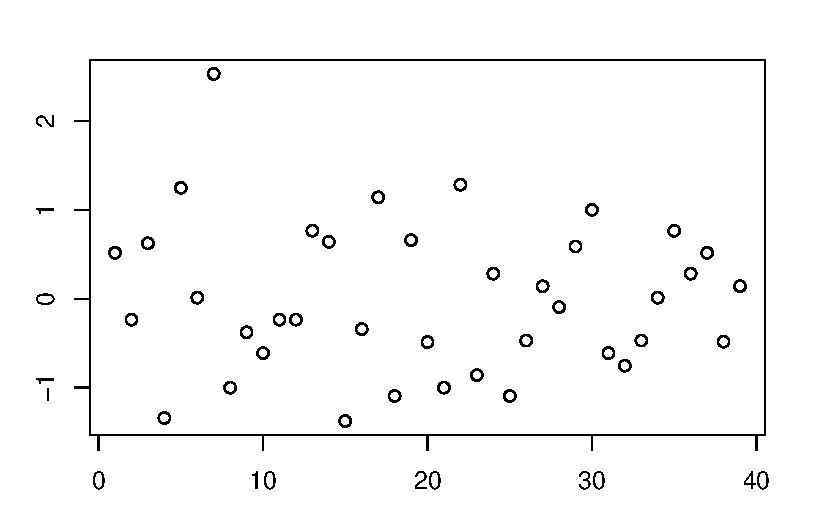
\includegraphics[keepaspectratio]{sta304_report_files/figure-pdf/unnamed-chunk-7-1.pdf}}
\end{center}

\begin{center}
\pandocbounded{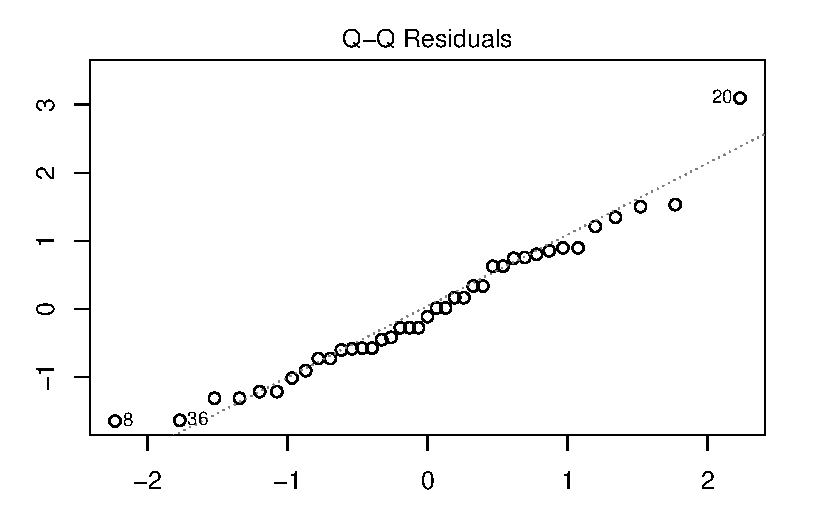
\includegraphics[keepaspectratio]{sta304_report_files/figure-pdf/unnamed-chunk-8-1.pdf}}
\end{center}

\begin{itemize}
\tightlist
\item
  Independence of errors: The residual plot shown above indicates no
  clear patterns, which suggests independence.
\item
  Normality of errors: Since the sample size is large, the Central Limit
  Theorem implies that the residuals should approximate a normal
  distribution. Also, a QQ-plot confirms approximate normality.
\item
  Homogeneity of variances: The residuals plot exhibits a roughly
  horizontal band, indicating constant variance across predicted values.
\item
  No multi-collinearity: We calculated the VIF of each independent
  variable, and found that
  \(VIF(\text{academic\_workload}) = 1.076844\), and
  \(VIF(\text{missed\_social\_events}) = 1.076844\). Since they are both
  less than \(5\), this indicates there is little correlation between
  them.
\end{itemize}

With all assumptions adequately met, we proceed with the regression
analysis.

\subsubsection{Computation and Statistical Test
Output}\label{computation-and-statistical-test-output-1}

The regression analysis produced the following results:

\begin{longtable}[]{@{}
  >{\raggedright\arraybackslash}p{(\linewidth - 8\tabcolsep) * \real{0.4118}}
  >{\raggedright\arraybackslash}p{(\linewidth - 8\tabcolsep) * \real{0.1765}}
  >{\raggedright\arraybackslash}p{(\linewidth - 8\tabcolsep) * \real{0.1471}}
  >{\raggedright\arraybackslash}p{(\linewidth - 8\tabcolsep) * \real{0.1324}}
  >{\raggedright\arraybackslash}p{(\linewidth - 8\tabcolsep) * \real{0.1324}}@{}}
\toprule\noalign{}
\begin{minipage}[b]{\linewidth}\raggedright
Statistic
\end{minipage} & \begin{minipage}[b]{\linewidth}\raggedright
Estimate
\end{minipage} & \begin{minipage}[b]{\linewidth}\raggedright
SE
\end{minipage} & \begin{minipage}[b]{\linewidth}\raggedright
t-value
\end{minipage} & \begin{minipage}[b]{\linewidth}\raggedright
\emph{p-value}
\end{minipage} \\
\midrule\noalign{}
\endhead
\bottomrule\noalign{}
\endlastfoot
Intercept (\(\beta_0\)) & 8.5521 & 0.6661 & 12.838 &
\(5.3 \times 10^{-15}\) \\
Slope 1 (\(\beta_1\)) & -0.1412 & 0.1666 & -0.848 & 0.40208 \\
Slope 2 (\(\beta_2\)) & -0.3763 & 0.1194 & -3.151 & 0.00327 \\
\end{longtable}

\begin{center}\rule{0.5\linewidth}{0.5pt}\end{center}

The residual standard error is \(0.864\) with \(36\) degrees of freedom.
The \(R^2\) value is \(0.2653\), the adjusted \(R^2\) is \(0.2245\), and
the F-statistic is \(F(2, 36) = 6.5\), with a \emph{p-value} of
\(0.003889\).

The equation of the regression line is given by: \[
\text{Hours of Sleep} = 8.5521 − 0.1412 \cdot \text{Academic Workload} - 0.3763 \cdot \text{Missed Social Events}
\]

\subsubsection{Interpretation}\label{interpretation-1}

The output of the regression analysis shows that the missed social
events has a statistically significant negative association with hours
of sleep (\(p = 0.00327\)). However, academic workload does not have a
significant relationship with hours of sleep (\(p = 0.40208\)).

\subsection{4.3.3. Research Question 3}\label{research-question-3}

\subsubsection{Relevant Graphs \&
Tables}\label{relevant-graphs-tables-2}

Research Question 3 examines whether mental health, represented by
stress levels, is affected by students' living situations and their
ability to maintain a work-life balance. To explore this relationship,
we first plot a boxplot of stress level by missed social events, with
students grouped by stress categories (``Always,'' ``Never,'' and
``Sometimes''). This plot suggests that students who miss social events
``Always'' or ``Sometimes'' have higher stress levels, while those who
``Never'' miss social events report lower stress levels.

\begin{center}
\pandocbounded{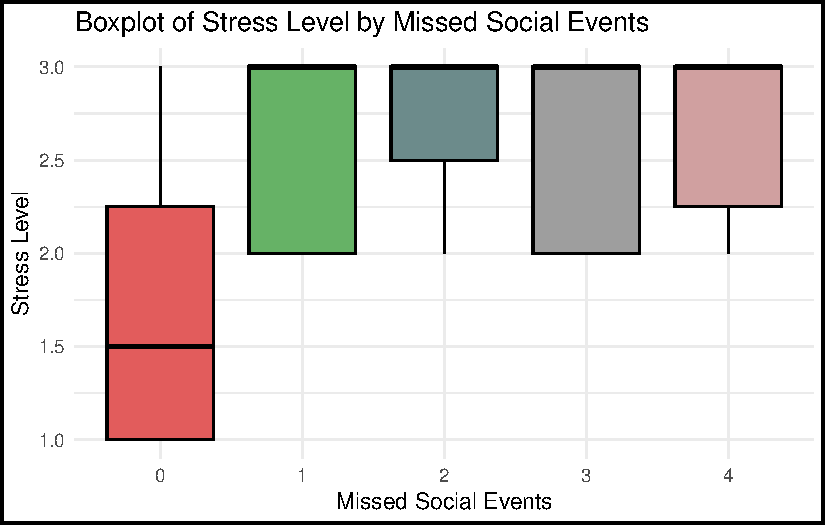
\includegraphics[keepaspectratio]{sta304_report_files/figure-pdf/unnamed-chunk-10-1.pdf}}
\end{center}

\subsubsection{Necessary Assumptions}\label{necessary-assumptions-2}

To investigate the impact of missed social events and living situations
on stress, we use a multiple linear regression model. The response
variable is stress (in numeric form), and the predictors are missed
social events and living situation. We verify the following assumptions:

\begin{center}
\pandocbounded{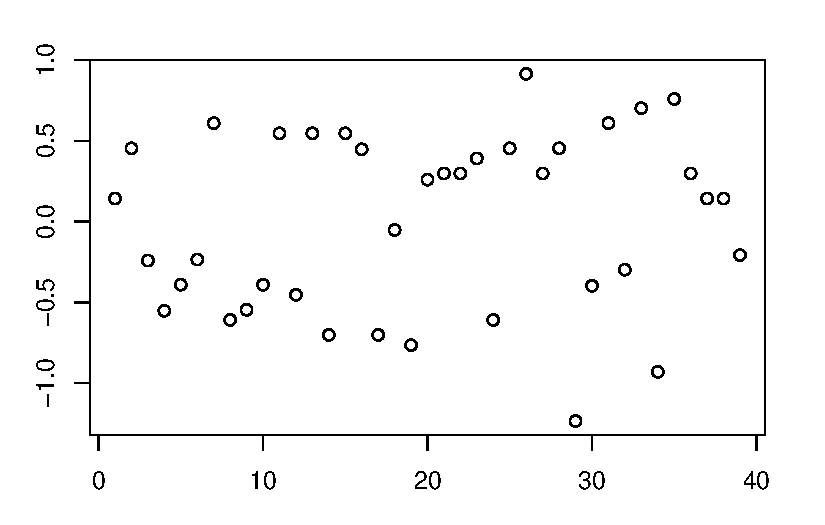
\includegraphics[keepaspectratio]{sta304_report_files/figure-pdf/unnamed-chunk-12-1.pdf}}
\end{center}

\begin{center}
\pandocbounded{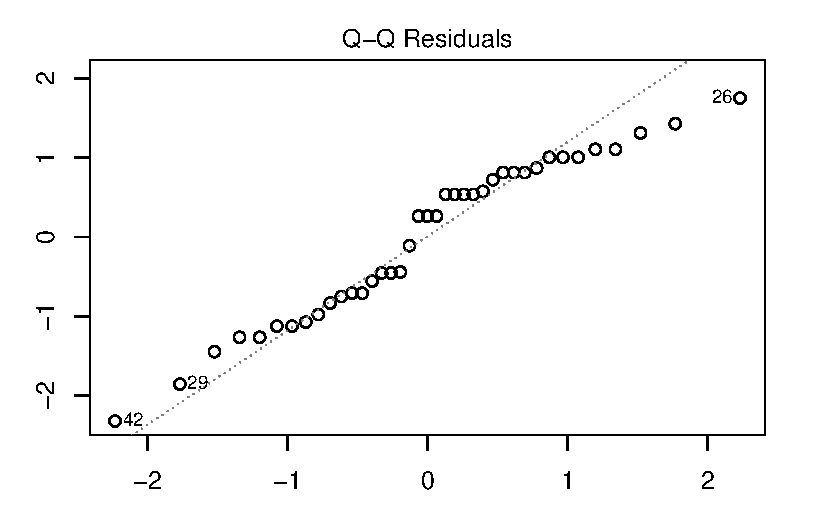
\includegraphics[keepaspectratio]{sta304_report_files/figure-pdf/unnamed-chunk-13-1.pdf}}
\end{center}

\begin{itemize}
\tightlist
\item
  Independence of errors: The residual plot indicates no clear patterns,
  suggesting that the errors are independent.
\item
  Normality of errors: Since the sample size is large, the Central Limit
  Theorem implies that the residuals should approximate a normal
  distribution. Also, a QQ-plot confirms approximate normality.
\item
  Homogeneity of variances: The residuals plot exhibits a roughly
  horizontal band, indicating constant variance across predicted values.
\item
  No multi-collinearity: We calculated the VIF of each independent
  variable, and found that
  \(VIF(\text{missed\_social\_events}) = 1.009045\), and
  \(VIF(\text{living\_situation}) = 1.003006\). Since both VIF values
  are close to \(1\), there's no indication of multicollinearity in this
  model.
\end{itemize}

With all assumptions adequately met, we proceed with the regression
analysis.

\subsubsection{Computation and Statistical Test
Output}\label{computation-and-statistical-test-output-2}

The regression analysis produced the following results:

\begin{longtable}[]{@{}
  >{\raggedright\arraybackslash}p{(\linewidth - 8\tabcolsep) * \real{0.4118}}
  >{\raggedright\arraybackslash}p{(\linewidth - 8\tabcolsep) * \real{0.1765}}
  >{\raggedright\arraybackslash}p{(\linewidth - 8\tabcolsep) * \real{0.1471}}
  >{\raggedright\arraybackslash}p{(\linewidth - 8\tabcolsep) * \real{0.1324}}
  >{\raggedright\arraybackslash}p{(\linewidth - 8\tabcolsep) * \real{0.1324}}@{}}
\toprule\noalign{}
\begin{minipage}[b]{\linewidth}\raggedright
Statistic
\end{minipage} & \begin{minipage}[b]{\linewidth}\raggedright
Estimate
\end{minipage} & \begin{minipage}[b]{\linewidth}\raggedright
SE
\end{minipage} & \begin{minipage}[b]{\linewidth}\raggedright
t-value
\end{minipage} & \begin{minipage}[b]{\linewidth}\raggedright
\emph{p-value}
\end{minipage} \\
\midrule\noalign{}
\endhead
\bottomrule\noalign{}
\endlastfoot
Intercept (\(\beta_0\)) & 1.93006 & 0.27980 & 6.898 &
\(6.02 \times 10^{-8}\) \\
Slope 1 (\(\beta_1\)) & 0.15560 & 0.07721 & 2.015 & 0.0518 \\
Slope 2 (\(\beta_2\)) & 0.81061 & 0.39928 & 2.030 & 0.0502 \\
Slope 3 (\(\beta_3\)) & 0.21206 & 0.28310 & 0.749 & 0.4590 \\
Slope 4 (\(\beta_4\)) & 0.30493 & 0.25406 & 1.200 & 0.2383 \\
\end{longtable}

\begin{center}\rule{0.5\linewidth}{0.5pt}\end{center}

The residual standard error is \(0.5745\) with \(34\) degrees of
freedom. The \(R^2\) value is \(0.1806\), the adjusted \(R^2\) value is
\(0.08416\), and the F-statistic is \(F(4, 34) = 1.873\), with a
\emph{p-value} of \(0.1378\).

The equation of the regression line is given by: \[
\begin{array}{lllllll}
\text{Stress} &=& 1.93006 &+& 0.15560 \cdot \text{Missed Social Events} &+& 0.81061 \cdot \text{Living On Campus} \\
              & &         &+& 0.21206 \cdot \text{Living With Family}   &+& 0.30493 \cdot \text{Living With Roommates}
\end{array}
\]

\subsubsection{Interpretation}\label{interpretation-2}

The results indicate that missed social events are a marginally
significant predictor of stress levels (\(p = 0.0518\)). Living
situation, specifically living on campus, is also a marginally
significant predictor (\(p = 0.0502\)). However, living with family
(\(p = 0.4590\)) and living with roommates (\(p = 0.2383\)) do not
significantly predict stress.

\section{5. Discussion and Results}\label{discussion-and-results}

For Research Question 1, we wished to investigate whether there is a
relationship between a student's academic workload and the prevalence of
mental health issues in students. Preliminarily, we plotted a boxplot to
look for any potential relationship between the two variables, and we
found that on average, students with higher stress levels tend to have a
higher academic workload. We later confirmed this with the simple linear
regression test and found that academic workload is a significant
predictor of stress.

For Research Question 2, we aimed to investigate whether there is a
relationship between students' academic workload and the amount of sleep
they get each night. An earlier test indicated no significant
relationship between hours of sleep and academic workload. Therefore, we
decided to examine the effect of another factor: the number of social
events a student misses on their hours of sleep. Initially, we plotted a
boxplot of hours of sleep against the number of missed social events.
The graph suggested that, on average, the more social events a student
misses, the fewer hours of sleep they tend to get. Our analysis
confirmed the earlier finding that academic workload does not have a
significant relationship with hours of sleep but also revealed a strong
relationship between the number of missed social events and students'
daily hours of sleep.

For Research Question 3, we studied whether mental health is affected by
students' living situations and their ability to maintain a work-life
balance. To explore this relationship, we first plotted a boxplot of
stress against the number of missed social events. The plot suggested
that students who sometimes or always miss social events tend to
experience more stress, while those who never miss social events
experience less stress. Then, we ran a test that concluded missing
social events and living on campus may slightly affect stress levels,
although the evidence is not very strong. In contrast, living with
family or roommates does not appear to have a significant impact on
stress.

ANOVA test between stress and academic workload has the calculated
F-value of 4.273, which is larger than the critical F-value of 2.960 at
the 5\% significance level with (3, 27) degrees of freedom. Therefore,
we reject the null hypothesis. There is a statistically significant
relationship between student academic workload and levels of stress.
This suggests that variations in academic workload are significantly
related to variations in stress.

ANOVA test between stress and hours of sleep has the calculated F-value
of 0.163, which is smaller than the critical F-value of 3.340 at the 5\%
significance level with (2, 28) degrees of freedom. Therefore, we fail
to reject the null hypothesis. There is no statistically significant
correlation between hours of sleep and levels of stress among students.
This suggests that variations in hours of sleep do not significantly
relate to variations in stress levels.

ANOVA test between stress and missed social events has the calculated
F-value of 1.092, which is smaller than the critical F-value of 2.649 at
the 5\% significance level with (4, 34) degrees of freedom. Therefore,
we fail to reject the null hypothesis. This means that stress levels and
missed social events do not have a significant relationship.

For the Chi-squared tests of independence between academic workload and
stress, anxiety, the respective \emph{p-value} are 0.0002288 and 0.0284
which are both less than \(\alpha=0.05\), so we reject the null
hypothesis. For the Chi-squared tests of independence between academic
workload and concentration, the p value is 0.3696, which is greater than
\(\alpha=0.05\), therefore we fail to reject the null hypothesis. This
suggests that a student's academic workload has and on their stress or
anxiety but not their concentration .

Chi-squared tests between students' living situation and their stress,
anxiety and concentration yield \emph{p-value} of 0.5446, 0.359, and
0.8241 respectively. All of these \emph{p-value} are greater than
\(\alpha=0.05\), therefore we fail to reject the null hypothesis for all
three of these Chi-squared tests. This suggests that the living
situation of a student doesn't have an association with their stress,
anxiety and concentration.

Chi-squared tests between students' time management skills and their
stress, anxiety and concentration yield \emph{p-value} of 0.2078,
0.5851, and 0.3151 respectively. All of these \emph{p-value} are greater
than \(\alpha=0.05\), therefore we fail to reject the null hypothesis
for all three of these Chi-squared tests. This suggests that a student's
ability to manage their time doesn't have an association with their
stress, anxiety and concentration.

Chi-squared tests between students' financials and their stress, anxiety
and concentration yield \emph{p-value} of 0.7223, 0.7236, and 0.6308
respectively. All of these \emph{p-value} are greater than
\(\alpha=0.05\), therefore we fail to reject the null hypothesis for all
three of these Chi-squared tests. This suggests that a student's
financial situation doesn't have an association with their stress,
anxiety and concentration.

The results of the multiple and linear regression tests indicate that
missed social events are a marginally significant predictor of stress
levels (p = 0.0518). Living situation, specifically living on campus, is
also a marginally significant predictor (p = 0.0502). However, living
with family (p = 0.4590) and living with roommates (p = 0.2383) do not
significantly predict stress.

Overall, the results of this study show that stress and anxiety among
university students is primarily related to academic factors, with
lifestyle factors such as sleep and socializing having less of an impact
than expected.

\section{6. Limitations}\label{limitations}

This experiment investigated the relationship between academic workload,
stress, sleep, and work life-balance among STA304 students. There were
many difficulties and limitations in conducting this experiment.

\subsection{Sampling}\label{sampling}

First, we used Simple Random Sampling (SRS) to sample the responses from
the survey, but we are not sure that randomness was guaranteed. Certain
students may have been more active in the survey, which may not
generalize the results. Therefore, various methods such as stratified
sampling could have been used instead of SRS. Also, there is a question
of voluntariness, because the students did not voluntarily participate
in the survey, but responded as part of their course participation.

\subsection{Questionnaire Design}\label{questionnaire-design}

We think that personal bias may occur due to the ambiguity of the
questions in the questionnaire, such as the mental health questions,
because they are not objective parameters that can be subjective to the
people who answer them. These parameters were measured indirectly in the
questionnaire, but this can increase the likelihood of measurement
error.

\subsection{Sample Size}\label{sample-size-1}

Third, there is the issue of sample size: while the sample size of this
experiment is relatively large compared to the population, the
population itself may be limited and the findings may not be
generalizable. We would expect the results to be more generalizable if
the experiment were conducted on a larger population. A larger
population would also allow for us to assume that all of our categorical
groups have a normal population distribution, one of the assumptions
needed for our ANOVA testing.

\section{7. Conclusion}\label{conclusion}

The linear regression analysis conducted for the three research
questions of this study provides valuable insights into the factors
affecting student stress and mental health. For Research Question 1, we
found a significant positive relationship between academic workload and
stress levels, suggesting that students with heavier workloads tend to
experience higher levels of stress. In Research Question 2, while
academic workload did not significantly impact the amount of sleep,
missed social events were found to significantly reduce hours of sleep,
which may contribute to poor mental health. For Research Question 3,
missed social events and living situations were marginally significant
predictors of stress, indicating that students who miss social events or
live on campus tend to report higher stress levels. These findings
highlight the importance of considering multiple factors in
understanding a student's overall well-being. However, the limitations
of this analysis, including potential issues with sample randomization
and measurement quality, should be addressed in future research to
enhance the robustness and accuracy of the results. Future studies
should also explore other possible variables, such as social support and
coping mechanisms, which may further explain the mental health
challenges faced by students.

Overall, the results of the ANOVA tests show that the stress levels of
the students sampled are primarily related to academic factors, with
lifestyle factors such as sleep and socializing having less of an impact
on their mental health than expected. In addition, this voluntary
response method was likely to result in selection bias.

For the Chi-squared tests of independence between academic workload and
stress, anxiety, the respective \emph{p-value} are 0.0002288 and 0.0284
which are both less than \(\alpha=0.05\), so we retain the null
hypothesis. For the Chi-squared tests of independence between academic
workload and concentration, the p value is 0.3696, which is greater than
\(\alpha=0.05\), therefore we reject the null hypothesis. This suggests
that a student's academic workload has an effect on their concentration
but not their stress or anxiety.

The linear regression analysis conducted for the three research
questions of this study provides valuable insights into the factors
affecting student stress and mental health. For Research Question 1, we
found a significant positive relationship between academic workload and
stress levels, suggesting that students with heavier workloads tend to
experience higher levels of stress. In Research Question 2, while
academic workload did not significantly impact the amount of sleep,
missed social events were found to significantly reduce hours of sleep,
which may contribute to poor mental health. For Research Question 3,
missed social events and living situations were marginally significant
predictors of stress, indicating that students who miss social events or
live on campus tend to report higher stress levels. These findings
highlight the importance of considering multiple factors in
understanding a student's overall well-being. However, the limitations
of this analysis, including potential issues with sample randomization
and measurement quality, should be addressed in future research to
enhance the robustness and accuracy of the results. Future studies
should also explore other possible variables, such as social support and
coping mechanisms, which may further explain the mental health
challenges faced by students.

\subsection{Documentation of AI Tool
Usage}\label{documentation-of-ai-tool-usage}

We utilized generative AI tools, namely ChatGPT, to help refine our
ideas and improve readability. These tools were used primarily for
brainstorming, grammar corrections, and the explanations of certain
sections. However, all the analytical work, including statistical
methods and interpretation of results, was done by the authors.

https://chatgpt.com/share/674a3a7d-83e4-8013-a381-4192bb2028da

\begin{enumerate}
\def\labelenumi{\arabic{enumi}.}
\item
  Beiter R, Nash R, McCrady M, Rhoades D, Linscomb M, Clarahan M, Sammut
  S. The prevalence and correlates of depression, anxiety, and stress in
  a sample of college students. J Affect Disord. 2015 Mar 1;173:90-6.
  doi:
  10.1016/j.jad.2014.10.054.(https://www.sciencedirect.com/science/article/abs/pii/S0165032714006867?via\%3Dihub).
  Epub 2014 Nov 8. PMID: 25462401.
\item
  Hysing M, Harvey AG, Linton SJ, Askeland KG, Sivertsen B. Sleep and
  academic performance in later adolescence: results from a large
  population-based study. J Sleep Res. 2016 Jun;25(3):318-24.
  \href{https://pubmed.ncbi.nlm.nih.gov/26825591/}{doi:10.1111/jsr.12373}.
  Epub 2016 Jan 30. PMID: 26825591.
\item
  Hershner SD, Chervin RD. Causes and consequences of sleepiness among
  college students. Nat Sci Sleep. 2014 Jun 23;6:73-84.
  \href{https://pmc.ncbi.nlm.nih.gov/articles/PMC4075951/}{doi:10.2147/NSS.S62907}.
  PMID: 25018659; PMCID: PMC4075951.
\end{enumerate}




\end{document}
